\documentclass[border=0.125cm]{standalone}
\usepackage{tikz}
\usepackage{pgfplots}
\usepackage{graphicx}

\usetikzlibrary{decorations.pathmorphing}
\pgfplotsset{compat=newest}
\usetikzlibrary{shapes.geometric,arrows,fit,matrix,positioning}
\tikzset{main node/.style={circle,fill=black!20,draw,minimum size=3.5mm,inner sep=0pt},
         every node/.style={circle,fill=black,draw,minimum size=1mm,inner sep=0pt,label distance=-1mm},
         subtree/.style={isosceles triangle,fill=blue!20,draw,minimum size=4mm,inner sep=0pt,shape border rotate=90},
         edge label/.style = {rectangle,draw=none,fill=none},
         blank edge/.style={edge from parent/.style={draw=none}},
         norm edge/.style={edge from parent/.style={black,thin,draw}},
}
\begin{document}
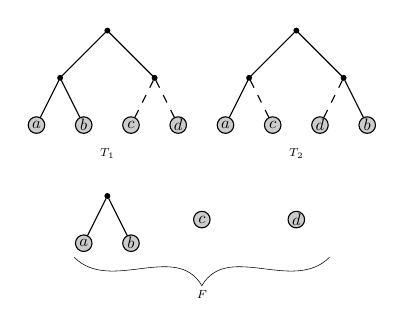
\begin{tikzpicture}[-,>=stealth', 
level 1/.style={sibling distance = 20mm},
level distance = 1cm, 
scale=0.6,
transform shape]

% \draw[help lines] (0,0) grid (8,-6);

\node (t1_0) at (2,0) {}
    child{
        [sibling distance = 10mm] node (t1_1) {}
            child{
                node [main node] (t1_2) {$a$}
            }
            child{
                node [main node] (t1_3) {$b$}
            }
    }
    child{
        [sibling distance = 10mm] node (t1_4) {}
            child[edge from parent path = {(\tikzparentnode ) -- (\tikzchildnode) [dashed]}]{
                node [main node] (t1_5) {$c$}
            }
            child[edge from parent path = {(\tikzparentnode ) -- (\tikzchildnode) [dashed]}]{
                node [main node] (t1_6) {$d$}
            }
    }
;

\node [edge label, xshift = 0mm, below=25mm, align=flush center] at (t1_0){
        \scriptsize{$T_1$}};

\node (t2_0) at (6,0) {}
    child{
         [sibling distance = 10mm]node (t2_1) {}
            child{
                node [main node] (t2_2) {$a$}
            }
            child[edge from parent path = {(\tikzparentnode ) -- (\tikzchildnode) [dashed]}]{
                node [main node] (t2_3) {$c$}
            }
    }
    child{
        [sibling distance = 10mm] node (t2_4) {}
            child[edge from parent path = {(\tikzparentnode ) -- (\tikzchildnode) [dashed]}]{
                node [main node] (t2_5) {$d$}
            }
            child{
                node [main node] (t2_6) {$b$}
            }
    }
;

\node [edge label, xshift = 0mm, below=25mm, align=flush center] at (t2_0){
        \scriptsize{$T_2$}};

% level 1/.style={sibling distance = 10mm}
\node[edge label] at (2,-2.5) {}
child[blank edge]{
    [sibling distance = 10mm]node (s1_0) {}
        child[norm edge]{
            node [main node] (s1_1) {$a$}
        }
        child[norm edge]{
            node [main node] (s1_2) {$b$}
        }
}
;

\node[main node] (s2_0) at (4,-4) {$c$};
\node[main node] (s3_0) at (6,-4) {$d$};

\node [edge label,  below=15mm, align=flush center] at (s2_0){
        \scriptsize{$F$}};

\draw[very thin] (1.3,-4.8) to [out=-45,in=120] (4,-5.4);
\draw[very thin] (6.7,-4.8) to [out=-135,in=60] (4,-5.4);

\end{tikzpicture}

\end{document}






